\documentclass[aspectratio=1610]{beamer}
\usetheme{Antibes}

\setbeamersize{text margin left=1em,text margin right=1em}

\usepackage{amsmath,amssymb,amsfonts}

\usepackage{siunitx}
\DeclareSIUnit\year{yr}

\graphicspath{{images}}

\title{Constraining the Volume of Earth's Early Oceans With a Temperature-Dependent Mantle Water Storage Capacity Model}
\author{Dong, J., Fischer, R. A., Stixrude, L. P., & Lithgow-Bertelloni, C. R.}
\institute{Columbia University}
\date{\today}

\begin{document}

\begin{frame}
      \titlepage
\end{frame}

\begin{frame}
      \frametitle{Outline}
      \tableofcontents
\end{frame}

\section{Major results of this paper}

\begin{frame}
      \frametitle{\secname}
      \begin{itemize}
            \item At the Earth's surface, the majority of water resides in the oceans, while
                  in the interior, major rock-forming minerals can incorporate significant
                  amounts of water as hydroxyl groups (OH), likely forming another reservoir
                  of water inside the planet.
            \item The water storage capacity (WSC) of Earth's mantle minerals generally
                  decreases at higher temperatures.
            \item Over billion-year timescales, the exchange of water between Earth's
                  interior and surface may control the surface oceans' volume change. They
                  calculated the WSC in Earth's solid mantle as a function of mantle
                  temperature.
            \item They find that WSC in a hot, early mantle $<$ the amount of water Earth's
                  mantle currently holds, so the additional water in the mantle today would
                  have resided on the surface of the early Earth and formed bigger oceans.
                  So the long-held assumption that the surface oceans' volume remained
                  nearly constant through geologic time may need to be reassessed.
      \end{itemize}
\end{frame}

\section{Introduction}

\begingroup  % See https://tex.stackexchange.com/a/213839/61591
\small
\begin{frame}
      \frametitle{\secname}
      \begin{itemize}
            \item The exact value of the present-day global net water flux into the deep
                  mantle is still under debate, the current estimates on it are on the order
                  of \SIrange{1e11}{1e12}{\kilo\gram\per\yr}. The onset and efficiency of
                  early subduction, and hence the total net water flux in the past, remains
                  even less constrained.
            \item Most of the existing geodynamical models did not take into account the
                  mineral physics constraints on mantle water storage; some assumed that the
                  solid mantle is a water reservoir with infinite storage capacity. When the
                  water content exceeds a rock's WSC, it will melt and release water.
            \item WSCs in major minerals of Earth's mantle have been studied individually by
                  high P-T experiments and/or ab-initio simulations. Although these
                  individual results have been obtained over wide ranges in T and P, a
                  detailed, quantitative estimate of the bulk mantle water storage capacity
                  is not yet available. So they estimate the bulk WSC in Earth's solid
                  mantle at different mantle potential temperatures ($T_p$) and demonstrates
                  that the bulk solid mantle WSC was smaller in the hotter mantle of the
                  early Earth relative to that of the present-day. They apply this
                  T-dependent water storage capacity model to constrain the volume of the
                  surface oceans and explore its implications on long-term sea-level change.
      \end{itemize}
\end{frame}
\endgroup

\section{Experimental data selection criteria}
\begin{frame}
      \frametitle{\secname}
      \begin{itemize}
            \item At least one liquid phase has to be present in the recovered phase assemblage to
                  ensure that the coexisting NAMs were most likely saturated with water (when the water
                  concentration equals the water storage capacity).
            \item Only water storage capacities measured by direct quantitative analytical methods
                  (Fourier transform infrared spectroscopy (FTIR), secondary ionization mass spectrometry
                  (SIMS), and elastic recoil detection analysis (ERDA)) were used. In contrast, those based on
                  more qualitative estimation methods (e.g., water content estimated from lattice parameters)
                  were excluded.
      \end{itemize}
\end{frame}

\section{Methods: water storage capacities in olivine}
\begin{frame}
      \frametitle{\secname}
      \begin{columns}
            \column{0.7\linewidth}
            \centering
            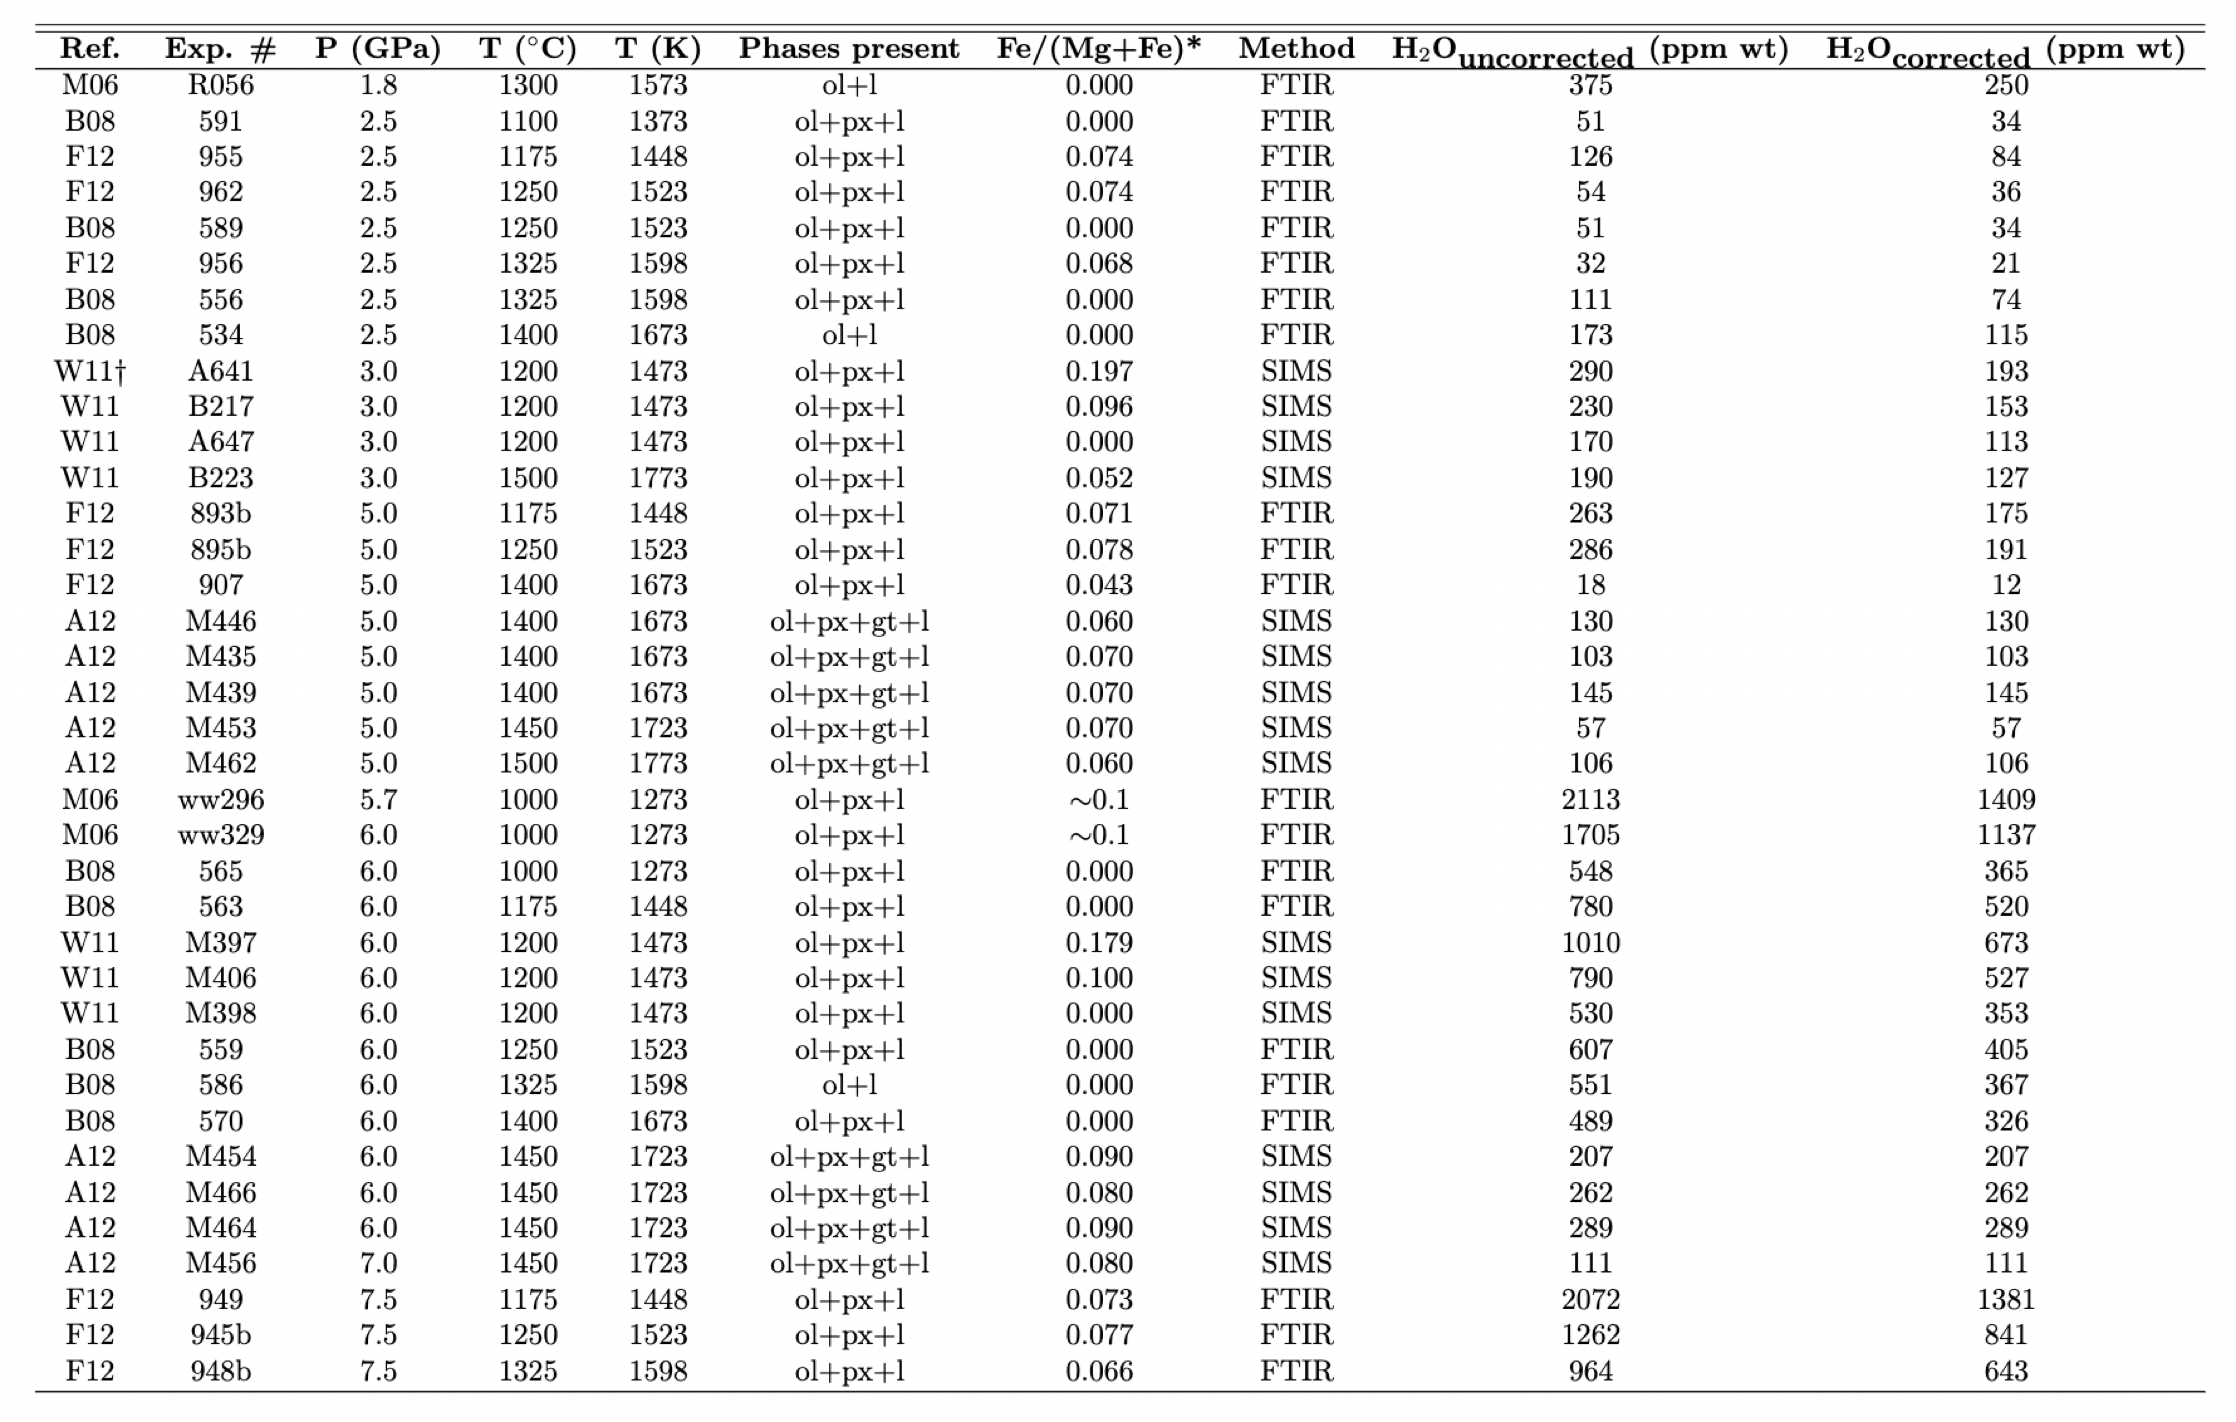
\includegraphics[width=\textwidth]{tab1.png}
            \caption{Summary of experimental data on water storage capacity in olivine}
            \column{0.3\linewidth}

      \end{columns}
\end{frame}

\end{document}
